\chapter{Introdução}
\label{chap:intro}
\thispagestyle{empty}

Este capítulo explica a motivação e objetivos deste projeto de otimização do desempenho em competições de um veículo elétrico protótipo de alta eficiência.
Apresenta a equipe de competição estudantil Milhagem UFMG onde este PFC foi realizado. E, também, descreve a estrutura desta monografia.

\section{Motivação e Justificativa}
\label{sec:motivacao}

A equipe Milhagem UFMG constrói protótipos de veículos para participar de competições
de eficiência energética. Atualmente a equipe possui dois veículos: o M84 equipado com um motor a combustão interna a gasolina e o DT1,
 apresentado na Figura \ref{fig:DT1}, que possui motor elétrico e bateria. As competições em que a
equipe participa são a Shell Eco-Marathon Brasil (nacional) e a Shell EcoMarathon Americas (internacional).
Nestas competições os veículos devem consumir a
menor quantidade de energia para percorrer trajeto, ou seja, devem ter a maior eficiência
energética.

\begin{figure}[h]
    \centering
    \caption{Veículo elétrico protótipo DT1}
    \label{fig:DT1}
    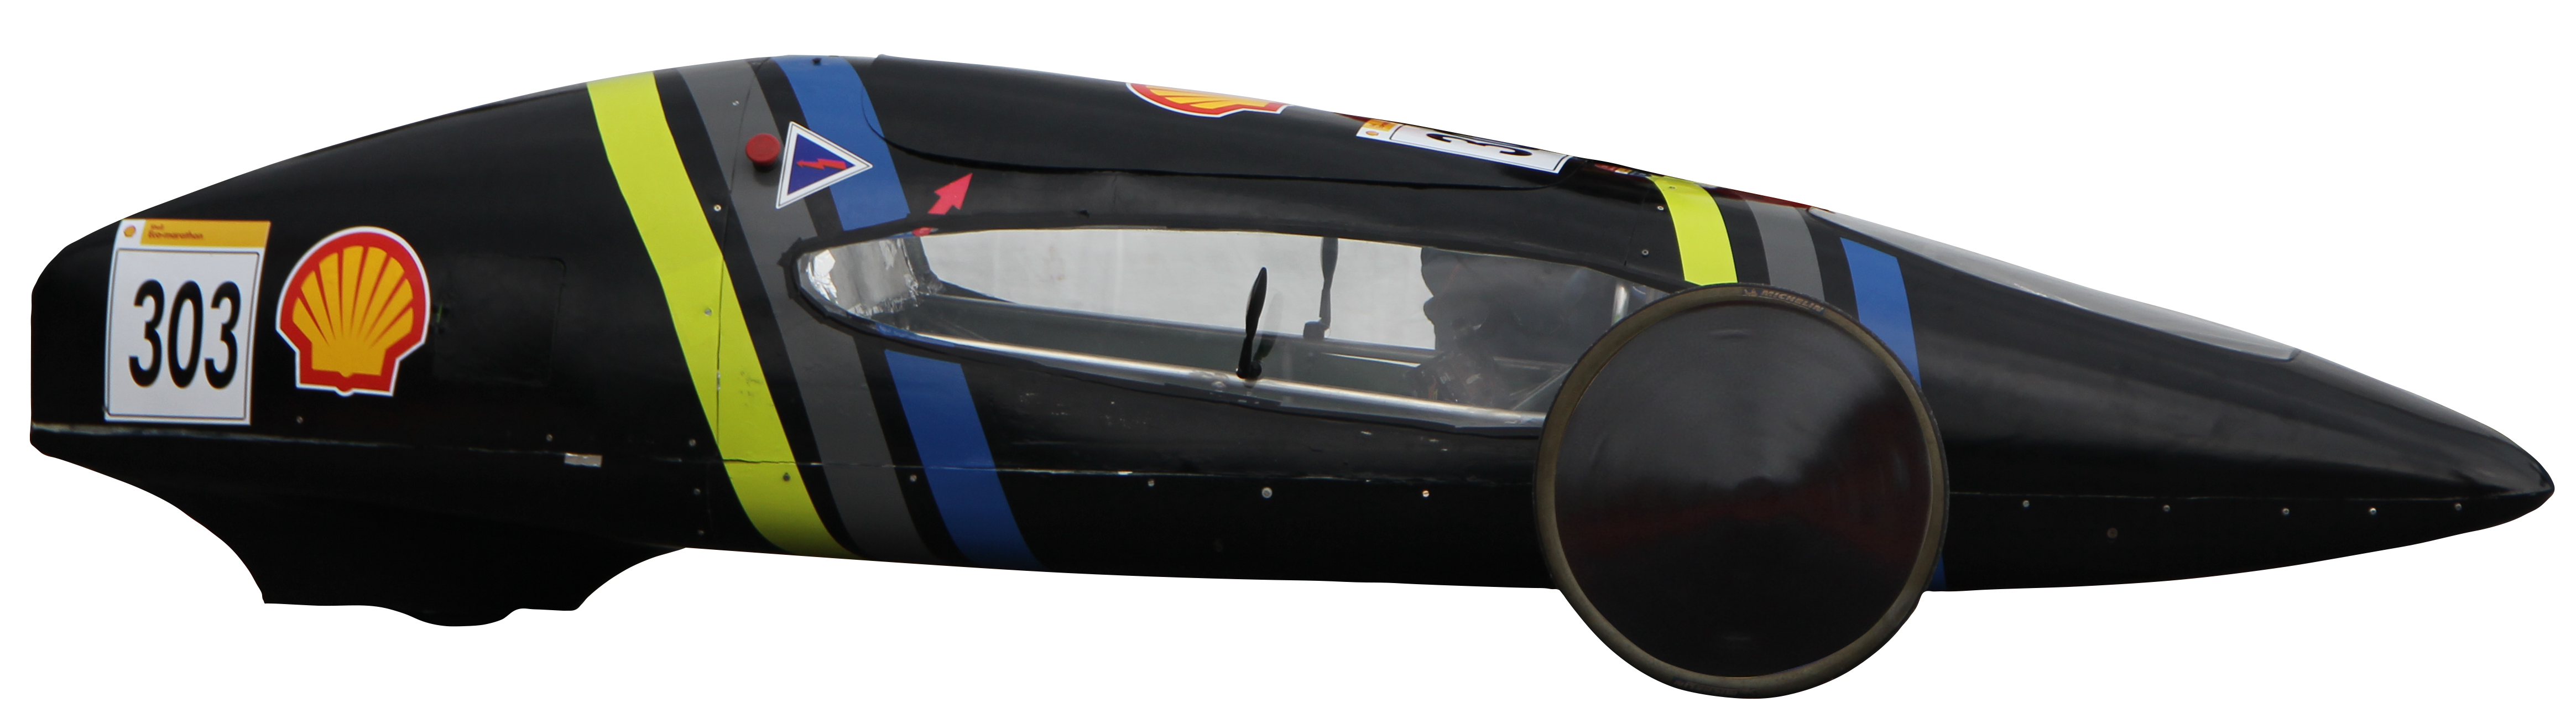
\includegraphics[scale=0.11]{Introducao/Figuras/dt1.png}
    \caption*{\footnotesize{Fonte: Equipe Milhagem UFMG}}
\end{figure}

Os principais fatores que influenciam no consumo de energia do veículo são a
aerodinâmica, o peso total, a resistência ao rolamento, o relevo do trajeto e a estratégia
de pista. Essa estratégia consiste na forma e nos momentos em que o motor deve ser
acionado. Um exemplo de uma estratégia de pista muito utilizada nesses protótipos é a
estratégia \textit{start-stop}, na qual o motor é desligado quando a velocidade é maior que 30
km/h e religado apenas quando é menor que 20 km/h, semelhante a um controle on-off
com histerese.

Durante a avaliação da eficiência energética de um protótipo ele deve seguir as seguintes
restrições: posições inicial e final fixas, velocidade inicial nula, velocidade instantânea
máxima e velocidade média mínima. Uma vez que essas restrições permitem inúmeras
estratégias de pista tem-se a necessidade encontrar a estratégia que maximize a
eficiência energética do veículo durante a avaliação de consumo.

% A teorias de controle ótimo fornece o embasamento para a
% que a estratégia de maior eficiência seja calculada numericamente. Para isso antes é necessário
%  a determinação do modelo matemático que represente o comportamento dinâmico do veículo.

\section{Objetivos do Projeto}
\label{sec:objetivos}

Tendo em vista o exposto acima, este projeto tem por objetivos direcionados ao protótipo DT1:

\begin{enumerate}[(a)]
    \item Definir o modelo matemático para a dinâmica do protótipo;
    \item Formular o problema de controle ótimo (OCP) pra obter a estratégia ótima;
    \item Implementar o algoritmo para solução desse OCP;
    \item Definir a estratégia ótima para a pista da Shell EcoMarathon Américas de 2019.
\end{enumerate}

\section{Local de Realização}
\label{sec:empresa}


Esse projeto foi desenvolvido na equipe de competição Milhagem UFMG, na qual o autor foi integrante de 2013 à 2015 e em 2018. A equipe é composta por alunos de graduação em engenharia de diversos períodos e sua sede é no Departamento de Engenharia Mecânica da UFMG.
Foi fundada, sobre orientação do
professor Paulo Iscold, em 2005 no Centro de Estudos Aeronáuticos (CEA) do qual fez
parte até 2006.
De 2006 a 2011 o projeto da equipe ficou suspenso retornando as atividades, sobre orientação do professor Fabrício Pujatti, no Centro de Tecnologia
de Mobilidade (CTM). A equipe ja desenvolveu 6 veículos, sendo DT1 o primeiro elétrico, e participou de 10 competições com os seguintes resultados:


\begin{itemize}
    \item Maratona Universitária de Eficiência Energética
          \begin{itemize}
              \item  Categoria gasolina
                    \begin{itemize}
                        \item 2005: 2º Lugar, com a marca de $227,6$ [km/L]
                        \item 2006: 1º Lugar, com a marca de $598,9$ [km/L]
                        \item 2011: 5º Lugar, com a marca de $199,0$ [km/L]
                        \item 2013: 4º Lugar, com a marca de $234,9$ [km/L]
                    \end{itemize}
          \end{itemize}
    \item Shell Eco-marathon Brasil
          \begin{itemize}
              \item  Categoria gasolina
                    \begin{itemize}
                        \item 2016: 2º Lugar, com a marca de $196,0$ [km/L]
                    \end{itemize}
              \item  Categoria elétrico
                    \begin{itemize}
                        \item 2017: 3º Lugar, com a marca de $315,6$ [km/kWh]
                        \item 2018: 1º Lugar, com a marca de $266,4$ [km/kWh]
                    \end{itemize}
          \end{itemize}
    \item Shell Eco-marathon Americas
          \begin{itemize}
              \item  Categoria elétrico
                    \begin{itemize}
                        \item 2018: 6º Lugar, com a marca de $266,5$ [km/kWh]
                        \item 2019: 2º Lugar, com a marca de $226,9$ [km/kWh]
                    \end{itemize}
          \end{itemize}
\end{itemize}

\section{Estrutura da Monografia}
\label{sec:organizacao}

Esta monografia está dividido em cinco capítulos. O presente capítulo apresentou uma introdução ao projeto a ser descrito nos capítulos seguintes. 
O Capítulo \ref{chap:revisao} é uma revisão bibliográfica que dos princípios básicos de modelagem veicular e controle ótimo de forma que abrange todos os
conceitos necessários para um melhor entendimento do projeto. O Capítulo \ref{chap:metodologia} aborda a metodologia de desenvolvimento do modelo matemático do DT1 e de implementação do software
para otimização da estratégia de pista. Os resultados obtidos no projeto são apresentados no Capítulo \ref{chap:resultados} e no 
capítulo \ref{chap:conclusao} tem-se a conclusão da monografia com algumas sugestões para trabalhos futuros e dificuldades encontradas durante a realização do projeto.

\clearpage